% Created by tikzDevice version 0.12.3.1 on 2021-04-09 21:52:41
% !TEX encoding = UTF-8 Unicode
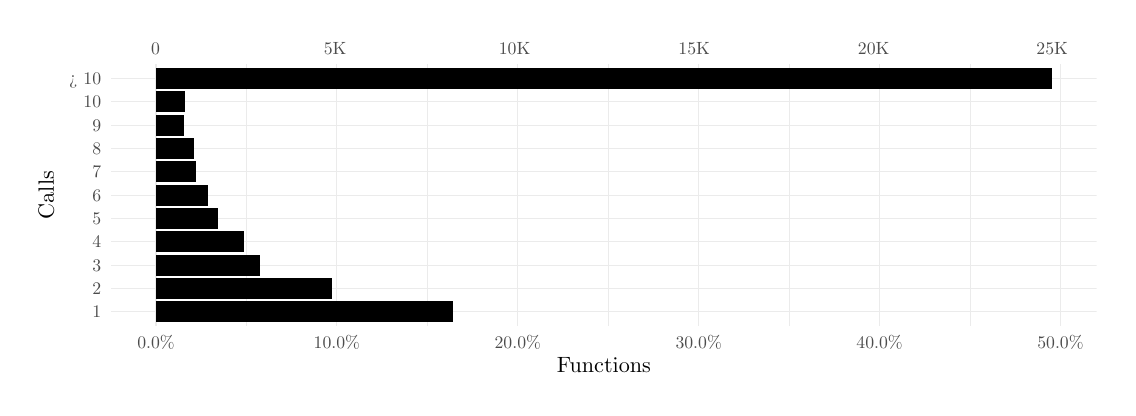
\begin{tikzpicture}[x=1pt,y=1pt]
\definecolor{fillColor}{RGB}{255,255,255}
\path[use as bounding box,fill=fillColor,fill opacity=0.00] (0,0) rectangle (390.26,130.09);
\begin{scope}
\path[clip] ( 30.17, 22.32) rectangle (386.26,116.83);
\definecolor{drawColor}{gray}{0.92}

\path[draw=drawColor,line width= 0.2pt,line join=round] ( 79.04, 22.32) --
	( 79.04,116.83);

\path[draw=drawColor,line width= 0.2pt,line join=round] (144.41, 22.32) --
	(144.41,116.83);

\path[draw=drawColor,line width= 0.2pt,line join=round] (209.77, 22.32) --
	(209.77,116.83);

\path[draw=drawColor,line width= 0.2pt,line join=round] (275.14, 22.32) --
	(275.14,116.83);

\path[draw=drawColor,line width= 0.2pt,line join=round] (340.51, 22.32) --
	(340.51,116.83);

\path[draw=drawColor,line width= 0.4pt,line join=round] ( 30.17, 27.38) --
	(386.26, 27.38);

\path[draw=drawColor,line width= 0.4pt,line join=round] ( 30.17, 35.82) --
	(386.26, 35.82);

\path[draw=drawColor,line width= 0.4pt,line join=round] ( 30.17, 44.26) --
	(386.26, 44.26);

\path[draw=drawColor,line width= 0.4pt,line join=round] ( 30.17, 52.70) --
	(386.26, 52.70);

\path[draw=drawColor,line width= 0.4pt,line join=round] ( 30.17, 61.14) --
	(386.26, 61.14);

\path[draw=drawColor,line width= 0.4pt,line join=round] ( 30.17, 69.58) --
	(386.26, 69.58);

\path[draw=drawColor,line width= 0.4pt,line join=round] ( 30.17, 78.01) --
	(386.26, 78.01);

\path[draw=drawColor,line width= 0.4pt,line join=round] ( 30.17, 86.45) --
	(386.26, 86.45);

\path[draw=drawColor,line width= 0.4pt,line join=round] ( 30.17, 94.89) --
	(386.26, 94.89);

\path[draw=drawColor,line width= 0.4pt,line join=round] ( 30.17,103.33) --
	(386.26,103.33);

\path[draw=drawColor,line width= 0.4pt,line join=round] ( 30.17,111.77) --
	(386.26,111.77);

\path[draw=drawColor,line width= 0.4pt,line join=round] ( 46.36, 22.32) --
	( 46.36,116.83);

\path[draw=drawColor,line width= 0.4pt,line join=round] (111.72, 22.32) --
	(111.72,116.83);

\path[draw=drawColor,line width= 0.4pt,line join=round] (177.09, 22.32) --
	(177.09,116.83);

\path[draw=drawColor,line width= 0.4pt,line join=round] (242.46, 22.32) --
	(242.46,116.83);

\path[draw=drawColor,line width= 0.4pt,line join=round] (307.82, 22.32) --
	(307.82,116.83);

\path[draw=drawColor,line width= 0.4pt,line join=round] (373.19, 22.32) --
	(373.19,116.83);
\definecolor{fillColor}{RGB}{0,0,0}

\path[fill=fillColor] ( 46.36,107.97) rectangle (370.07,115.57);

\path[fill=fillColor] ( 46.36, 23.58) rectangle (153.52, 31.18);

\path[fill=fillColor] ( 46.36, 99.53) rectangle ( 56.78,107.13);

\path[fill=fillColor] ( 46.36, 32.02) rectangle (109.88, 39.62);

\path[fill=fillColor] ( 46.36, 40.46) rectangle ( 83.98, 48.06);

\path[fill=fillColor] ( 46.36, 48.90) rectangle ( 78.12, 56.49);

\path[fill=fillColor] ( 46.36, 57.34) rectangle ( 68.81, 64.93);

\path[fill=fillColor] ( 46.36, 65.78) rectangle ( 65.03, 73.37);

\path[fill=fillColor] ( 46.36, 74.22) rectangle ( 60.74, 81.81);

\path[fill=fillColor] ( 46.36, 82.66) rectangle ( 60.20, 90.25);

\path[fill=fillColor] ( 46.36, 91.10) rectangle ( 56.47, 98.69);
\end{scope}
\begin{scope}
\path[clip] (  0.00,  0.00) rectangle (390.26,130.09);
\definecolor{drawColor}{gray}{0.30}

\node[text=drawColor,anchor=base,inner sep=0pt, outer sep=0pt, scale=  0.64] at ( 46.21,120.43) {0};

\node[text=drawColor,anchor=base,inner sep=0pt, outer sep=0pt, scale=  0.64] at (111.09,120.43) {5K};

\node[text=drawColor,anchor=base,inner sep=0pt, outer sep=0pt, scale=  0.64] at (175.96,120.43) {10K};

\node[text=drawColor,anchor=base,inner sep=0pt, outer sep=0pt, scale=  0.64] at (240.83,120.43) {15K};

\node[text=drawColor,anchor=base,inner sep=0pt, outer sep=0pt, scale=  0.64] at (305.70,120.43) {20K};

\node[text=drawColor,anchor=base,inner sep=0pt, outer sep=0pt, scale=  0.64] at (370.22,120.43) {25K};
\end{scope}
\begin{scope}
\path[clip] (  0.00,  0.00) rectangle (390.26,130.09);
\definecolor{drawColor}{gray}{0.30}

\node[text=drawColor,anchor=base east,inner sep=0pt, outer sep=0pt, scale=  0.64] at ( 26.57, 25.18) {1};

\node[text=drawColor,anchor=base east,inner sep=0pt, outer sep=0pt, scale=  0.64] at ( 26.57, 33.62) {2};

\node[text=drawColor,anchor=base east,inner sep=0pt, outer sep=0pt, scale=  0.64] at ( 26.57, 42.05) {3};

\node[text=drawColor,anchor=base east,inner sep=0pt, outer sep=0pt, scale=  0.64] at ( 26.57, 50.49) {4};

\node[text=drawColor,anchor=base east,inner sep=0pt, outer sep=0pt, scale=  0.64] at ( 26.57, 58.93) {5};

\node[text=drawColor,anchor=base east,inner sep=0pt, outer sep=0pt, scale=  0.64] at ( 26.57, 67.37) {6};

\node[text=drawColor,anchor=base east,inner sep=0pt, outer sep=0pt, scale=  0.64] at ( 26.57, 75.81) {7};

\node[text=drawColor,anchor=base east,inner sep=0pt, outer sep=0pt, scale=  0.64] at ( 26.57, 84.25) {8};

\node[text=drawColor,anchor=base east,inner sep=0pt, outer sep=0pt, scale=  0.64] at ( 26.57, 92.69) {9};

\node[text=drawColor,anchor=base east,inner sep=0pt, outer sep=0pt, scale=  0.64] at ( 26.57,101.13) {10};

\node[text=drawColor,anchor=base east,inner sep=0pt, outer sep=0pt, scale=  0.64] at ( 26.57,109.57) {> 10};
\end{scope}
\begin{scope}
\path[clip] (  0.00,  0.00) rectangle (390.26,130.09);
\definecolor{drawColor}{gray}{0.30}

\node[text=drawColor,anchor=base,inner sep=0pt, outer sep=0pt, scale=  0.64] at ( 46.36, 14.31) {0.0{\%}};

\node[text=drawColor,anchor=base,inner sep=0pt, outer sep=0pt, scale=  0.64] at (111.72, 14.31) {10.0{\%}};

\node[text=drawColor,anchor=base,inner sep=0pt, outer sep=0pt, scale=  0.64] at (177.09, 14.31) {20.0{\%}};

\node[text=drawColor,anchor=base,inner sep=0pt, outer sep=0pt, scale=  0.64] at (242.46, 14.31) {30.0{\%}};

\node[text=drawColor,anchor=base,inner sep=0pt, outer sep=0pt, scale=  0.64] at (307.82, 14.31) {40.0{\%}};

\node[text=drawColor,anchor=base,inner sep=0pt, outer sep=0pt, scale=  0.64] at (373.19, 14.31) {50.0{\%}};
\end{scope}
\begin{scope}
\path[clip] (  0.00,  0.00) rectangle (390.26,130.09);
\definecolor{drawColor}{RGB}{0,0,0}

\node[text=drawColor,anchor=base,inner sep=0pt, outer sep=0pt, scale=  0.80] at (208.22,  5.56) {Functions};
\end{scope}
\begin{scope}
\path[clip] (  0.00,  0.00) rectangle (390.26,130.09);
\definecolor{drawColor}{RGB}{0,0,0}

\node[text=drawColor,rotate= 90.00,anchor=base,inner sep=0pt, outer sep=0pt, scale=  0.80] at (  9.51, 69.58) {Calls};
\end{scope}
\end{tikzpicture}
